\chapter{Evaluación de Clasificadores}
Después de tener cargado el nuevo almacenamiento de datos con la información homogeneizada, se procedió a evaluar los algoritmos de clasificación para elegir los más confiables para construir la interfaz de consultas, que permita conocer los posibles resultados de un evaluado.

El objetivo de este trabajo de grado era entregar información sobre los posibles resultados de un estudiante en cada una de las áreas académicas evaluadas por la prueba Saber 11\degree. Estas áreas son en total 14, así que para cada una de estas áreas se debió construir un clasificador que predijera con el mayor índice de confianza el resultado a obtener por el evaluado. (En el anexo D se encuentra información sobre como interpretar los resultados de la prueba).
\section{Selección de atributos}
El primer paso para la construcción de estos clasificadores fue filtrar la cantidad de atributos predictores disponibles. Al momento de realizar esta fase se contaba con 78 atributos predictores, varios de estos atributos constaban con una gran cantidad de registros nulos, ya que la frecuencia con la que se almacenó en las bases de datos fue muy baja.

Para la selección de estos atributos a ser filtrados se evaluó primero la cantidad de veces en las que este fue registrado, y utilizando la suite de algoritmos de minera de datos Weka\footnote{\url{http://www.cs.waikato.ac.nz/ml/weka/}} se realizó un filtro de selección de atributos utilizando algoritmos especializados para esta tarea.
\subsection{Selección manual}
La tabla \ref{tab:cuadro15} muestra los atributos que se seleccionaron de manera manual, el criterio para esta primera selección fue que al menos estuvieran presentes en 12 (50\%) de las bases de datos consultadas.

\begin{table}[!Hhtb]
\centering
\begin{tabular}{|p{0.5cm}|p{8cm}|p{1.8cm}|}
\hline
	\rowcolor[gray]{0.9} 
	\textbf{ID} &
	\textbf{Atributo} &
	\textbf{Cantidad}\\
\hline
4 & COLE_CODIGO_MCPIO* & 24 \\ \hline
6 & COLE\_INST\_JORNADA & 24 \\ \hline
7 & COLE\_INST\_VLR\_PENSION & 24 \\ \hline
36 & ESTU\_DISC\_MOTRIZ & 24 \\ \hline
37 & ESTU\_DISC\_SORDO\_CON\_INTERPRETE & 24 \\ \hline
38 & ESTU\_DISC\_SORDO\_SIN\_INTERPRETE & 24 \\ \hline
41 & ESTU\_EDAD & 24 \\ \hline
47 & ESTU\_GENERO & 24 \\ \hline
35 & ESTU\_DISC\_INVIDENTE & 22 \\ \hline
44 & ESTU\_EXAM\_DEPTO\_PRESENTACION & 22 \\ \hline
51 & ESTU\_RESIDE\_DEPTO & 22 \\ \hline
1 & COLE\_CALENDARIO\_COLEGIO & 17 \\ \hline
2 & COLE\_CARACTER\_COLEGIO & 17 \\ \hline
48 & ESTU\_IES\_RAZON\_DESEADA & 17 \\ \hline
49 & ESTU\_CARR\_RAZON\_DESEA & 17 \\ \hline
55 & ESTU\_TRABAJA & 17 \\ \hline
58 & FAMI\_COD\_EDUCA\_MADRE & 17 \\ \hline
59 & FAMI\_COD\_EDUCA\_PADRE & 17 \\ \hline
60 & FAMI\_COD\_OCUP\_MADRE & 17 \\ \hline
61 & FAMI\_COD\_OCUP\_PADRE & 17 \\ \hline
63 & FAMI\_ING\_FMILIAR\_MENSUAL & 17 \\ \hline
68 & FAMI\_NUM\_PERS\_GRUP\_FAM & 17 \\ \hline
3 & COLE\_DEPTO\_COLEGIO & 16 \\ \hline
5 & COLE\_IDIOMA\_COLEGIO & 15 \\ \hline
43 & ESTU\_ETNIA & 15 \\ \hline
46 & ESTU\_EXAM\_MPIO\_PRESENTACION & 15 \\ \hline
52 & ESTU\_RESIDE\_MPIO & 15 \\ \hline
54 & ESTU\_TIPO\_DOC & 14 \\ \hline
\end{tabular}
\caption{Atributos predictores seleccionados de manera manual.}
\label{tab:cuadro15}
\end{table}
\begin{quote}
* Originalmente el atributo registrado 24 veces era COLE_INST_NOMBRE, pero como este tenía alrededor de 12500 opciones, se volvió complicado trabajar con él, por lo tanto se decidió utilizar este para conocer el municipio al que el colegio pertenece y así el atributo COLE_CODIGO_MCPIO se pudo registrar las 24 veces.
\end{quote}
Tras aplicar este primer filtro la cantidad de atributos predictores considerados útiles, se redujo a 28.
Después, usando estos 28 atributos, se procedió a utilizar los algoritmos de selección de atributos predictores disponibles en Weka.
\subsection{Selección automática}
Weka brinda la capacidad de realizar esta selección de atributos utilizando métodos evaluadores que se dividen en 2 tipos: los evaluadores de subconjuntos y los prorrateadores de atributos. El primer tipo se encarga de evaluar cual subconjunto de datos es el mejor para predecir la clase, este utiliza un método de búsqueda del tipo forward o backward. El segundo tipo no evalúa subconjuntos, si no que asigna a cada atributo un valor que indica el nivel de correlación que posee con la clase a predecir, este al contrario de utilizar un método de búsqueda, utiliza un ranker para indicar la importancia de cada atributo.

El primer paso para poder utilizar Weka fue construir los archivos arff\footnote{\url{http://weka.wikispaces.com/ARFF}} estos son los archivos que usa Weka para transmitir la información a los algoritmos. En la primera prueba se construyó un archivo arff con 1000 registros, con los datos obtenidos desde el almacenamiento de datos construido en el capítulo anterior. La idea de realizar esta prueba inicial era determinar los tiempos que demoraba cada posible combinación entre los métodos de evaluación y los métodos de búsqueda que ofrece Weka. Después de realizar esta prueba se optó por la utilización de 6 combinaciones que fueron las que lograron manipular la cantidad de datos presentados, en un tiempo aceptable, teniendo en cuenta que más adelante se ejecutarían pruebas con archivos que contenían hasta 500.000 registros.

La razón para que algunas combinaciones no fueran seleccionadas, fue porque nunca se logró obtener una solución en el tiempo otorgado (20 minutos) o lanzaron error al momento de procesar el archivo. El tiempo de 20 minutos, fue tomado como un límite justificable, ya que de los algoritmos de los cuales si se obtuvo respuesta, no tomaron un tiempo mayor a 3 minutos.

La tabla \ref{tab:cuadro16} muestra las combinaciones seleccionadas.

Como ya se explicó que se construyó un clasificador por cada área evaluada, la selección de atributos también se aplicó a cada una de estas clases a predecir, es decir que por cada área se crearon los archivos arff para ser analizados en los algoritmos.

Los archivos ARFF creados para realizar cada prueba fueron construidos seleccionando de manera aleatoria registros de la base de datos homogeneizada. Además estos archivos fueron creados con distintas cantidades de registros, con el fin de tener una mejor visión sobre el comportamiento de los algoritmos a medida que se aumentaba la cantidad de registros. Estas cantidades fueron 1.000, 10.000, 100.000 y 500.000. Es decir, por cada área evaluada se crearon 4 archivos arff que fueron ejecutados en las 6 combinaciones distintas, dando así 24 evaluaciones a analizar. 

\begin{table}[!Hhtb]
\centering
\begin{tabular}{|p{1cm}|p{6cm}|p{6cm}|}
\hline
	\rowcolor[gray]{0.9}
	\textbf{ID} &
	\textbf{Método de evaluación} &
	\textbf{Método de búsqueda}\\
\hline
1 & CfsSubsetEval\protect\footnotemark & BestFirst\protect\footnotemark \\ \hline
2 & CfsSubsetEval  & GeneticSearch\protect\footnotemark  \\ \hline
3 & CfsSubsetEval  & GreedyStepwise\protect\footnotemark \\ \hline
4 & ClassifierSubsetEval\protect\footnotemark & GeneticSearch \\ \hline
5 & GainRatioAttributeEval\protect\footnotemark & Ranker\protect\footnotemark \\ \hline
6 & InfoGainAttributeEval\protect\footnotemark & Ranker  \\ \hline
\end{tabular}
\caption{Combinaciones utilizadas en Weka para seleccionar atributos predictores.}
\label{tab:cuadro16}
\end{table}
\addtocounter{footnote}{-7}
\footnotetext{\url{http://weka.sourceforge.net/doc.stable/weka/attributeSelection/CfsSubsetEval.html}}
\addtocounter{footnote}{1}
\footnotetext{\url{http://weka.sourceforge.net/doc.stable/weka/attributeSelection/BestFirst.html}}
\addtocounter{footnote}{1}
\footnotetext{\url{http://weka.sourceforge.net/doc.stable/weka/attributeSelection/GeneticSearch.html}}
\addtocounter{footnote}{1}
\footnotetext{\url{http://weka.sourceforge.net/doc.stable/weka/attributeSelection/GreedyStepwise.html}}
\addtocounter{footnote}{1}
\footnotetext{\url{http://weka.sourceforge.net/doc.stable/weka/attributeSelection/ClassifierSubsetEval.html}}
\addtocounter{footnote}{1}
\footnotetext{\url{http://weka.sourceforge.net/doc.stable/weka/attributeSelection/GainRatioAttributeEval.html}}
\addtocounter{footnote}{1}
\footnotetext{\url{http://weka.sourceforge.net/doc.stable/weka/attributeSelection/Ranker.html}}
\addtocounter{footnote}{1}
\footnotetext{\url{http://weka.sourceforge.net/doc.stable/weka/attributeSelection/InfoGainAttributeEval.html}}
\section{Creación de vistas minables}
Posterior a la ejecución de los algoritmos de selección automática, se reevaluó la calidad de los atributos predictores y su capacidad de ser realmente aportantes al momento de predecir el posible puntaje en un área académica. Se decidió que los atributos ESTU_EXAM_MPIO_PRESENTACION y ESTU_EXAM_DEPTO_PRESENTACION no serían tenidos en cuenta para la construcción de los clasificadores, ya que al analizar la base de datos, en más del 90\% de los casos el valor de estos 2 atributos era equivalente al valor de los atributos COLE_CODIGO_MCPIO y COLE_DEPTO_COLEGIO respectivamente, por lo tanto se generaba redundancia en los datos y esto ocasiona que la calidad de las predicciones disminuya. 

También el atributo ESTU_TIPO_DOC que indica el tipo de documento con el que la persona se inscribió, no entregaba información realmente útil. Al analizar la base de datos alrededor del 95\% de los registros se dividían entre ``Tarjeta de Identidad'' o “Cedula de Ciudadanía”, los otros valores posibles no eran comunes. Este atributo se solapa con el atributo ESTU_EDAD, ya que el valor “Tarjeta de Identidad” los tenían los evaluados menores de 18 años y “Cedula de Ciudadanía” los evaluadores mayores de 18 años. Por lo tanto, es claro que conociendo la edad de un evaluado, se puede conocer qué tipo de documento utiliza, así que la edad absorbió este atributo y por eso no fue tenido en cuenta a la hora de construir los clasificadores.

Después de analizar los resultados de la ejecución de los algoritmo de selección de atributos, se procedió a construir las vistas minables que iban a ser procesadas en cada uno de los algoritmos de construcción de clasificadores.

Para la construcción de estas vista minables, se realizó una selección entre los 28 atributos filtrados inicialmente y los atributos que tuvieron una mayor presencia en los resultados de los algoritmos de selección de atributos. En algunas áreas se crearon 2 vistas minables para tener una mejor perspectiva, respecto a distintos comportamientos. No se definió un límite mínimo de selección de los atributos en los resultados de los algoritmos, la cantidad de atributos que compone cada vista minable se decidió teniendo en cuenta el número de veces que fue seleccionado el más frecuente.

Los procesos de minería de datos involucran, además de los algoritmos, el conocimiento que se tenga sobre el problema, en ocasiones algunos atributos pueden no ser relevantes al momento de ejecutar los algoritmos, pero es conocido por las personas involucradas en el proceso, que estos atributos sí determinan un factor importante en el caso de estudio. Teniendo en cuenta este criterio, algunos atributos que tuvieron poca relevancia en los algoritmos de selección, fueron escogidos para ser predictores, ya que se consideró que su significado podría beneficiar la calidad de las predicciones.

La tabla \ref{tab:cuadro31} muestra los atributos procesados en los algoritmos de selección de atributos, para el caso del área de biología, y la frecuencia con la que los algoritmos de selección le dieron importancia. Cabe aclarar que en el caso de los algoritmos de evaluación que utilizan un método de búsqueda “Ranker” siempre aparecieron todos los valores, pero la puntuación asignada a algunos de ellos era de 0.0 por lo tanto estos no se contaron como atributos seleccionados por ese algoritmo.

\begin{table}[!Hhtb]
\centering
\begin{tabular}{|p{1cm}|p{8cm}|p{3cm}|}
\hline
	\rowcolor[gray]{0.9}
	\textbf{ID} &
	\textbf{Atributo} &
	\textbf{\# de veces que se seleccionó}\\
\hline
58    & FAMI_COD_EDUCA_MADRE & 19 \\
\hline
4     & COLE_CODIGO_MCPIO & 17 \\
\hline
41    & ESTU_EDAD & 17 \\
\hline
63    & FAMI_ING_FMILIAR_MENSUAL & 17 \\
\hline
6     & COLE_INST_JORNADA & 16 \\
\hline
52    & ESTU_RESIDE_MPIO & 16 \\
\hline
7     & COLE_INST_VLR_PENSION & 15 \\
\hline
59    & FAMI_COD_EDUCA_PADRE & 15 \\
\hline
60    & FAMI_COD_OCUP_MADRE & 15 \\
\hline
51    & ESTU_RESIDE_DEPTO & 12 \\
\hline
3     & COLE_DEPTO_COLEGIO & 8 \\
\hline
38    & ESTU_DISC_SORDO_SIN_INTERPRETE & 8 \\
\hline
43    & ESTU_ETNIA & 7 \\
\hline
61    & FAMI_COD_OCUP_PADRE & 7 \\
\hline
5     & COLE_IDIOMA_COLEGIO & 6 \\
\hline
47    & ESTU_GENERO & 6 \\
\hline
49    & ESTU_CARR_RAZON_DESEA & 6 \\
\hline
48    & ESTU_IES_RAZON_DESEADA & 5 \\
\hline
36    & ESTU_DISC_MOTRIZ & 4 \\
\hline
37    & ESTU_DISC_SORDO_CON_INTERPRETE & 4 \\
\hline
1     & COLE_CALENDARIO_COLEGIO & 3 \\
\hline
35    & ESTU_DISC_INVIDENTE & 3 \\
\hline
2     & COLE_CARACTER_COLEGIO & 2 \\
\hline
68    & FAMI_NUM_PERS_GRUP_FAM & 2 \\
\hline
55    & ESTU_TRABAJA & 1 \\
\hline
\end{tabular}
\caption{Cantidad de veces que los atributos fueron seleccionados como buenos predictores por los algoritmos de selección de atributos, en el área de biología.}
\label{tab:cuadro31}
\end{table}
En la tabla \ref{tab:cuadro31} se observa los atributos ordenados con base a la relevancia que tuvieron en los algoritmos de selección. Para crear las vistas minables se seleccionaron los de mayor frecuencia.

El criterio aplicado, en el caso de biología, a la selección de los atributos fue que estos se encontraran en al menos 12 de las combinaciones, es decir en el 50\% de estas, 10 atributos cumplieron con este criterio.

Después de analizar estos primeros 10 atributos se pudo notar que existían 2 que indicaban la misma información pero con diferente granularidad, estos eran COLE_DEPTO_COLEGIO y COLE_CODIGO_MCPIO, ambos indican la ubicación del colegio, uno a nivel departamental y el otro a nivel municipal, por lo tanto solo era necesario seleccionar uno de ellos para indicar la ubicación del colegio. Pero como los 2 tenían una frecuencia que cumplía con el criterio, se decidió crear 2 vista minables en donde una tuviera una granularidad de departamento en la ubicación del colegio y la otra una granularidad de municipio en la ubicación del colegio.

Así, siguiendo una lógica similar a la aplicada al área de biología, se crearon las vistas minables de las demás áreas académicas.

En las 14 áreas académicas se intentó seguir las mismas reglas de manera general, pero en algunas áreas como por ejemplo medio ambiente, eran pocos los atributos que cumplían con estar seleccionado en al menos 12 combinaciones, en el caso de medio ambiente, solo 3 atributos cumplían esto.
 
También para el caso de algunos atributos, como FAMI_COD_OCUP_PADRE, no tuvieron buena frecuencia de selección, pero FAMI_COD_OCUP_MADRE si lo hizo, teniendo en cuenta que estos indican la misma información de los padres, en algunas vistas minables se agregó la ocupación del padre como atributo a pesar de que su frecuencia de selección no fuera alta.

La tabla \ref{tab:cuadro32} muestra las vistas minables creadas para cada una de las áreas académicas.

\begin{table}[!Hhtb]
\centering
\begin{tabular}{|p{3.5cm}|p{7cm}|}
\hline
	\rowcolor[gray]{0.9} 
	\multicolumn{2}{|c|}{
	\textbf{Vistas minables}}\\
\hline
	\rowcolor[gray]{0.5}
	Nombre & Atributos\\
\hline
Biologia9 & 6, 7, 41, 51, 58, 59, 60, 61, 63 \\
\hline
Biologia10 & 4, 6, 7, 41, 52, 58, 59, 60, 61, 63 \\
\hline
Filosofia7 & 1, 4, 7, 41, 52, 58, 59 \\
\hline
Fisica11 & 1, 4, 7, 41, 47, 52, 58, 59, 60, 61, 63 \\
\hline
Fisica112 & 1, 6, 7, 41, 47, 52, 58, 59, 60, 61, 63 \\
\hline
Ingles11 & 4, 5, 6, 7, 41, 52, 58, 59, 60, 61, 63 \\
\hline
Lenguaje10 & 4, 7, 41, 43, 52, 58, 59, 60, 61, 63 \\
\hline
Lenguaje102 & 4, 6, 7, 41, 43, 58, 59, 60, 61, 63 \\
\hline
Matematica10 & 4, 6, 7, 41, 47, 52, 58, 59, 60, 61 \\
\hline
Matematica102 & 1, 3, 6, 7, 41, 47, 58, 59, 60, 61 \\
\hline
MedioAmbiente5 & 2, 4, 52, 58, 60 \\
\hline
MedioAmbiente7 & 2, 4, 52, 58, 59, 60, 61 \\
\hline
ProBiologia6 & 1, 4, 7, 58, 60, 63 \\
\hline
ProBiologia8 & 1, 4, 7, 58, 59, 60, 61, 63 \\
\hline
ProLenguaje7 & 2, 4, 7, 41, 58, 60, 63 \\
\hline
ProLenguaje9 & 2, 4, 7, 41, 58, 59, 60, 61, 63 \\
\hline
ProMatematica7 & 4, 6, 7, 41, 58, 60, 63 \\
\hline
ProMatematica9 & 4, 6, 7, 41, 58, 59, 60, 61, 63 \\
\hline
ProSociales7 & 1, 4, 7, 41, 58, 60, 63 \\
\hline
ProSociales9 & 1, 4, 7, 41, 58, 59, 60, 61, 63 \\
\hline
Quimica10 & 4, 6, 7, 41, 52, 58, 59, 60, 61, 63 \\
\hline
Sociales7 & 4, 7, 41, 52, 58, 60, 63  \\
\hline
Sociales9 & 4, 7, 41, 52, 58, 59, 60, 61, 63  \\
\hline
Violencia11 & 4, 6, 7, 41, 52, 55, 58, 59, 60, 61, 63 \\
\hline
\end{tabular}
\caption{Lista de las vistas minables creadas.}
\label{tab:cuadro32}
\end{table}
Teniendo lista la estructura para construir las vistas minables, se procedió a la carga de estas. Cada vista minable se creó con 1.000, 10.000 y 100.000 registros.

Las vistas minables se cargaron utilizando el lenguaje de programación Python. Se utilizó el generador de números aleatorios para seleccionar los registros en la base de datos de manera que se aseguró que no existía ninguna correlación entre los registros cargados. También se aseguró que estos registros fueran cargados sin ninguno de sus atributos con valor nulo, esto se hizo con el fin de que los algoritmos de clasificación tuvieran una mejor confiabilidad.

En el caso de las profundizaciones, en donde la cantidad de registros es menor, ya que la presentación de estas pruebas es opcional, no se pudieron crear vistas minables de 100.000 registros, porque fue difícil lograr que todos los atributos coincidieran en no ser nulos, por eso en las profundizaciones los grupos fueron de 1.000, 10.000 y 50.000.

Con las vistas minables cargadas, se procedió a la evaluación de estos en los algoritmos de construcción de clasificadores.
\section{Construcción de clasificadores}
Utilizando Weka, se procedió a generar distintos clasificadores, con base en los anteriores trabajos revisados y que sirvieron de apoyo para este, los algoritmos seleccionados para evaluar las vistas minables fueron: generador de árboles de decisión C4.5\cite{key-170}, K vecinos más cercanos\cite{key-180}, Naive Bayes\cite{key-190} y red neuronal RBF (Radial Basis Function)\cite{key-200}.

Weka ofrece la posibilidad de ejecutar cada uno de estos algoritmos con una colección de datos de entrenamiento y evaluar su nivel de confianza con un archivo de evaluación.

Los archivos de entrenamiento fueron aquellos que se crearon siguiendo la estructura de las vistas minables presentadas en la anterior sección. En Weka es posible dividir estos archivos, para que un porcentaje sea de entrenamiento y el otro porcentaje sea de evaluación. Pero en este trabajo se decidió crear los archivos de evaluación a partir de un conjunto de datos completamente nuevo y desconocido para el conjunto de datos de entrenamiento, esto se logró utilizando los resultados de la prueba en el año 2012. 

Como se había explicado inicialmente, en el momento de iniciar este trabajo las bases de datos disponibles eran las de los años 2000 hasta 2011, pero en el momento de iniciar la creación de los clasificadores, la base de datos del año 2012 estaba disponible para su descarga y se pudo utilizar como un conjunto de datos desconocido para el conjunto de datos inicial.

Para cada vista minable se creó un archivo que tenía la misma estructura pero que se cargaba con registros de la base de datos de 2012, estos archivos de evaluación se crearon con una cantidad de 1000 registros. Es decir que por cada clasificador creado, se evaluaba su precisión con 1000 registros de los cuales se conocía la clase, pero al clasificador se le presentaba como desconocida, para que la predijera.

La precisión se calculó de manera lineal, por ejemplo si en los archivos de evaluación se tenía un registro con calificación, en alguna de las áreas académicas, de F (entre 50 y 60 puntos) y el clasificador lo asignaba en la clase F, entonces se entendía como un 100\% de éxito en la predicción. En el caso de que el clasificador lo asignara en la clase E, se entendía como un 90\% de éxito, ya que se trabajó con 10 niveles y en este caso el error de un nivel es un 10\% menos de confianza en la precisión. Así, si por ejemplo, se hubiera predicho en la clase B el nivel de confianza era de 60\%.

Con estas evaluaciones para visualizar el nivel de confianza que ofrecía cada clasificador, fue que se tomó la decisión de cuales clasificadores iban a ser utilizados en la construcción de la interfaz de consultas.

A continuación se presentan los resultados de cada algoritmo construido con cada una de las vistas minables definidas para predecir cada área académica.
\subsection{Generador de árboles de decisión C4.5}
El algoritmo de árboles de clasificación C4.5 se encuentra implementado en Weka en la librería J48\footnote{\url{http://weka.sourceforge.net/doc.stable/weka/classifiers/trees/J48.html}}.

Un árbol de decisión es un conjunto de condiciones organizadas en una estructura jerárquica. De tal manera que la decisión final se puede tomar siguiendo las condiciones desde la raíz hasta alguna de las hojas.

El problema de la construcción de un árbol puede ser explicado de una manera recursiva, Primero se selecciona un atributo para ser ubicado en la raíz del árbol, y se crea una rama por cada posible valor que puede tomar este atributo. Esto divide el conjunto de datos de entrenamiento en distintas secciones con cada valor del nodo raíz. Y el proceso se repite de manera recursiva por cada una de las nuevas ramas, usando las instancias que están presentes en cada nuevo nodo. La condición de parada es cuando todas las instancias en un nodo tiene la misma clasificación\cite{key-210}.
\begin{figure}[H]
\begin{centering}
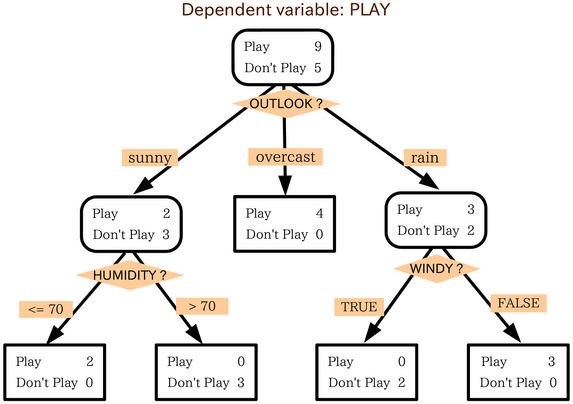
\includegraphics[scale=0.6]{c45}
\par\end{centering}
\caption{Representación gráfica de un árbol de decisión.}
\end{figure}
El algoritmo, se entrenó y evaluó con cada una de las vistas minables de las áreas académicas, los resultados obtenidos, en cada uno de los clasificadores, se muestran en la tabla \ref{tab:cuadro33}.\\

\begin{longtable}{|p{3cm}|p{3cm}|p{2cm}|p{2cm}|p{2cm}|p{2cm}|}
%\centering
%\begin{tabular}{|p{3cm}|p{3cm}|p{2cm}|p{2cm}|p{2cm}|p{2cm}|}
\hline
	\rowcolor[gray]{0.5} 
	\multicolumn{2}{|c|}{Vista minable} &
	\multicolumn{4}{|c|}{Porcentaje de éxito de las instancias clasificadas}\\
	\hline
	\rowcolor[gray]{0.9} 
	Nombre & \# de instancias & 100\% & 90\% & 80\% & 70\%\\
	\hline
	\endhead
	\hline
	\multicolumn{6}{r}{\textit{Continua en la siguiente pagina.}} \\
	\endfoot
	\endlastfoot
	\multirow{3}[5]{*}{Biologia9} & 1000  & 445   & 481   & 67    & 7\\
\cline{2-6}      & 10000 & 445   & 481   & 67    & 7 \\
\cline{2-6}      & 100000 & 453   & 481   & 59    & 7 \\
\hline
\multirow{3}[6]{*}{Biologia10} & 1000  & 496   & 434   & 65    & 4 \\
\cline{2-6}      & 10000 & 496   & 434   & 65    & 4 \\
\cline{2-6}      & 100000 & 499   & 433   & 63    & 4 \\
\hline
\multirow{3}[6]{*}{Filosofia7} & 1000  & 399   & 490   & 93    & 17 \\
\cline{2-6}      & 10000 & 399   & 490   & 93    & 17 \\
\cline{2-6}      & 100000 & 399   & 490   & 93    & 17 \\
\hline
\multirow{3}[6]{*}{Fisica11} & 1000  & 540   & 400   & 56    & 2 \\
\cline{2-6}      & 10000 & 540   & 400   & 56    & 2 \\
\cline{2-6}      & 100000 & 540   & 400   & 56    & 2 \\
\hline
\multirow{3}[6]{*}{Fisica112} & 1000  & 517   & 419   & 60    & 4 \\
\cline{2-6}      & 10000 & 517   & 419   & 60    & 4 \\
\cline{2-6}      & 100000 & 517   & 419   & 60    & 4 \\
\hline
\multirow{2}[4]{*}{Ingles11} & 1000  & 428   & 417   & 80    & 40 \\
\cline{2-6}      & 10000 & 519   & 329   & 80    & 12 \\
\hline
\multirow{3}[6]{*}{Lenguaje10} & 1000  & 548   & 406   & 44    & 1 \\
\cline{2-6}      & 10000 & 548   & 406   & 44    & 1 \\
\cline{2-6}      & 100000 & 509   & 432   & 56    & 2 \\
\hline
\multirow{3}[6]{*}{Lenguaje102} & 1000  & 580   & 392   & 25    & 3 \\
\cline{2-6}      & 10000 & 580   & 392   & 25    & 3 \\
\cline{2-6}      & 100000 & 580   & 392   & 25    & 3 \\
\hline
\multirow{3}[6]{*}{Matematica10} & 1000  & 356   & 519   & 97    & 18 \\
\cline{2-6}      & 10000 & 356   & 519   & 97    & 18 \\
\cline{2-6}      & 100000 & 356   & 519   & 97    & 18 \\
\hline
\multirow{3}[6]{*}{Matematica102} & 1000  & 346   & 508   & 108   & 25 \\
\cline{2-6}      & 10000 & 346   & 508   & 108   & 25 \\
\cline{2-6}      & 100000 & 346   & 508   & 108   & 25 \\
\hline
\multirow{3}[6]{*}{MedioAmbiente5} & 1000  & 0     & 847   & 148   & 0 \\
\cline{2-6}      & 10000 & 0     & 847   & 148   & 0 \\
\cline{2-6}      & 100000 & 0     & 847   & 148   & 0 \\
\hline
\multirow{3}[6]{*}{MedioAmbiente7} & 1000  & 4     & 851   & 144   & 0 \\
\cline{2-6}      & 10000 & 4     & 851   & 144   & 0 \\
\cline{2-6}      & 100000 & 4     & 851   & 144   & 0 \\
\hline
\multirow{3}[6]{*}{ProBiologia6} & 1000  & 285   & 426   & 258   & 25 \\
\cline{2-6}      & 10000 & 263   & 417   & 279   & 34 \\
\cline{2-6}      & 50000 & 263   & 417   & 279   & 34 \\
\hline
\multirow{3}[6]{*}{ProBiologia8} & 1000  & 314   & 396   & 242   & 40 \\
\cline{2-6}      & 10000 & 314   & 396   & 242   & 40 \\
\cline{2-6}      & 50000 & 280   & 404   & 254   & 53 \\
\hline
\multirow{3}[6]{*}{ProLenguaje7} & 1000  & 207   & 559   & 223   & 10 \\
\cline{2-6}      & 10000 & 207   & 559   & 223   & 10 \\
\cline{2-6}      & 50000 & 207   & 559   & 223   & 10 \\
\hline
\multirow{3}[6]{*}{ProLenguaje9} & 1000  & 221   & 545   & 221   & 8 \\
\cline{2-6}      & 10000 & 221   & 545   & 221   & 8 \\
\cline{2-6}      & 50000 & 221   & 545   & 221   & 8 \\
\hline
\multirow{3}[6]{*}{ProMatematica7} & 1000  & 176   & 697   & 87    & 31 \\
\cline{2-6}      & 10000 & 176   & 697   & 87    & 31 \\
\cline{2-6}      & 50000 & 232   & 653   & 78    & 28 \\
\hline
\multirow{3}[6]{*}{ProMatematica9} & 1000  & 157   & 686   & 101   & 48 \\
\cline{2-6}      & 10000 & 157   & 686   & 101   & 48 \\
\cline{2-6}      & 50000 & 160   & 684   & 101   & 47 \\
\hline
\multirow{3}[6]{*}{ProSociales7} & 1000  & 184   & 600   & 205   & 9 \\
\cline{2-6}      & 10000 & 184   & 600   & 205   & 9 \\
\cline{2-6}      & 50000 & 213   & 517   & 224   & 38 \\
\hline
\multirow{3}[6]{*}{ProSociales9} & 1000  & 174   & 605   & 211   & 7 \\
\cline{2-6}      & 10000 & 174   & 605   & 211   & 7 \\
\cline{2-6}      & 50000 & 188   & 554   & 220   & 33 \\
\hline
\multirow{3}[6]{*}{Quimica10} & 1000  & 640   & 328   & 30    & 2 \\
\cline{2-6}      & 10000 & 640   & 328   & 30    & 2 \\
\cline{2-6}      & 100000 & 640   & 328   & 30    & 2 \\
\hline
\multirow{3}[6]{*}{Sociales7} & 1000  & 474   & 439   & 81    & 5 \\
\cline{2-6}      & 10000 & 474   & 439   & 81    & 5 \\
\cline{2-6}      & 100000 & 474   & 439   & 81    & 5 \\
\hline
\multirow{3}[6]{*}{Sociales9} & 1000  & 466   & 457   & 70    & 4 \\
\cline{2-6}      & 10000 & 466   & 457   & 70    & 4 \\
\cline{2-6}      & 100000 & 466   & 457   & 70    & 4 \\
\hline
\multirow{3}[6]{*}{Violencia11} & 1000  & 457   & 424   & 104   & 14 \\
\cline{2-6}      & 10000 & 457   & 424   & 104   & 14 \\
\cline{2-6}      & 100000 & 457   & 424   & 104   & 14 \\
\hline
%\end{tabular}
\caption{Resultados de la construcción y evaluación de las vistas minables usando el algoritmo C4.5.}
\label{tab:cuadro33}
\end{longtable}
En la tabla \ref{tab:cuadro33} se puede observar que todos los clasificadores, creados con cada una de las vistas minables, tuvieron más del 70\% de éxito en al menos el 90\% de las instancias presentadas en los archivos de evaluación.

También se resalta, que en varias de las vistas minables, la cantidad de registros con los que se entrenó el clasificador, no causaron un diferencia en la precisión de este.

Los clasificadores obtenidos usando el algoritmo C4.5 tuvieron un grado de confianza considerablemente positivo, pero la estabilidad presentada al momento de cambiar la cantidad de registro, causó desconfianza sobre la calidad de la precisión. 
Al analizar los arboles generados por los algoritmos, se encontró que los arboles solo se generaban con un nodo, que inmediatamente clasificaba la clase a la que pertenecía la instancia. Esta clase era la que más veces se encontraba en el archivo de evaluación.

Por ejemplo, el archivo de entrenamiento Biologia9 con 1.000 registros, contenía 579 instancias en la clase E, 228 en la clase F y 158 en la clase D. Al procesar el algoritmo con este archivo, el árbol generado, solo tenía un nodo donde todas las instancias de evaluación, se clasificaban en la clase E. Por lo tanto, estos resultados, solo asignan una predicción basándose en la clase mayoritariamente encontrada en las instancias de entrenamiento, así que su confianza no es realmente significativa.\\
\subsection{K vecinos más cercanos}
El algoritmo de los K vecinos más cercanos se encuentra implementado en Weka en la librería IBK\footnote{\url{http://weka.sourceforge.net/doc.stable/weka/classifiers/lazy/IBk.html}}.

La regla del vecino más cercano es simple, este asigna a la instancia que se quiere clasificar, la clase del ejemplo más próximo utilizando una función de distancia. Esta función usualmente es la función de distancia Euclidiana, aunque una alternativa también frecuentemente usada es la función de distancia Manhattan.

El problema con esta sencilla manera de clasificar las instancias, es que toma mucho tiempo comparar, cada una de las instancias de entrenamiento con la instancia a clasificar, para determinar cuál es la más cercana. La manera de reducir el tiempo que toma esta comparación es representando los datos de entrenamiento como un árbol, este árbol es llamado un kD-tree\cite{key-220}, porque almacena un grupo de puntos en un espacio k-dimensional. Siendo k el número de atributos de las instancias.

El uso de los kD-tree ha ayudado a solucionar el problema de la comparación uno por uno, ya que el árbol divide el espacio en dimensiones que agrupan instancias con atributos similares, así cada evaluación no debe compararse contra cada instancia, sino que se compara contra las dimensiones, y se asigna a la clase de la dimension con la que tuvo una mayor similitud\cite{key-210}.

Se procedió a ejecutar el algoritmo con 2 distintas configuraciones para obtener los clasificadores de cada vista minable. Una configuración utilizó un valor de K=1 el cual indicaba la cantidad de vecinos mas cercanos que se iban a buscar para asignar un valor a la instancia evaluada. La otra configuración usó este valor en K=2. Los resultados de la configuración con K=1 se muestra en la tabla \ref{tab:cuadro34} y los resultados con K=2 en la tabla \ref{tab:cuadro35}.\\

\begin{longtable}{|p{3cm}|p{3cm}|p{2cm}|p{2cm}|p{2cm}|p{2cm}|}
%\centering
%\begin{tabular}{|p{3cm}|p{3cm}|p{2cm}|p{2cm}|p{2cm}|p{2cm}|}
\hline
	\rowcolor[gray]{0.5} 
	\multicolumn{2}{|c|}{Vista minable} &
	\multicolumn{4}{|c|}{Porcentaje de éxito de las instancias clasificadas}\\
	\hline
	\rowcolor[gray]{0.9} 
	Nombre & \# de instancias & 100\% & 90\% & 80\% & 70\%\\
	\hline
	\endhead
	\hline
	\multicolumn{6}{r}{\textit{Continua en la siguiente pagina.}} \\
	\endfoot
	\endlastfoot
\multirow{3}[5]{*}{Biologia9} & 1000  & 345   & 495   & 143   & 16 \\
\cline{2-6}      & 10000 & 387   & 469   & 129   & 12 \\
\cline{2-6}      & 100000 & 388   & 476   & 115   & 17 \\
\hline
\multirow{3}[6]{*}{Biologia10} & 1000  & 416   & 469   & 99    & 14 \\
\cline{2-6}      & 10000 & 447   & 447   & 95    & 9 \\
\cline{2-6}      & 100000 & 442   & 453   & 96    & 8 \\
\hline
\multirow{3}[6]{*}{Filosofia7} & 1000  & 369   & 470   & 131   & 27 \\
\cline{2-6}      & 10000 & 362   & 482   & 125   & 29 \\
\cline{2-6}      & 100000 & 359   & 487   & 130   & 20 \\
\hline
\multirow{3}[6]{*}{Fisica11} & 1000  & 424   & 456   & 109   & 10 \\
\cline{2-6}      & 10000 & 427   & 446   & 111   & 14 \\
\cline{2-6}      & 100000 & 416   & 473   & 100   & 10 \\
\hline
\multirow{3}[6]{*}{Fisica112} & 1000  & 394   & 470   & 115   & 19 \\
\cline{2-6}      & 10000 & 413   & 454   & 118   & 12 \\
\cline{2-6}      & 100000 & 449   & 445   & 92    & 13 \\
\hline
\multirow{2}[4]{*}{Ingles11} & 1000  & 192   & 278   & 200   & 194 \\
\cline{2-6}      & 10000 & 204   & 267   & 202   & 162 \\
\hline
\multirow{3}[6]{*}{Lenguaje10} & 1000  & 412   & 474   & 106   & 7 \\
\cline{2-6}      & 10000 & 452   & 457   & 83    & 7 \\
\cline{2-6}      & 100000 & 457   & 451   & 84    & 7 \\
\hline
\multirow{3}[6]{*}{Lenguaje102} & 1000  & 417   & 448   & 115   & 17 \\
\cline{2-6}      & 10000 & 374   & 476   & 124   & 22 \\
\cline{2-6}      & 100000 & 395   & 470   & 110   & 24 \\
\hline
\multirow{3}[6]{*}{Matematica10} & 1000  & 337   & 470   & 144   & 37 \\
\cline{2-6}      & 10000 & 353   & 454   & 144   & 35 \\
\cline{2-6}      & 100000 & 332   & 497   & 125   & 35 \\
\hline
\multirow{3}[6]{*}{Matematica102} & 1000  & 282   & 420   & 215   & 59 \\
\cline{2-6}      & 10000 & 280   & 445   & 201   & 54 \\
\cline{2-6}      & 100000 & 296   & 421   & 199   & 63 \\
\hline
\multirow{3}[6]{*}{MedioAmbiente5} & 1000  & 237   & 656   & 101   & 0 \\
\cline{2-6}      & 10000 & 222   & 670   & 101   & 0 \\
\cline{2-6}      & 100000 & 196   & 692   & 105   & 0 \\
\hline
\multirow{3}[6]{*}{MedioAmbiente7} & 1000  & 285   & 626   & 85    & 0 \\
\cline{2-6}      & 10000 & 211   & 673   & 115   & 0 \\
\cline{2-6}      & 100000 & 229   & 671   & 98    & 0 \\
\hline
\multirow{3}[6]{*}{ProBiologia6} & 1000  & 212   & 383   & 301   & 89 \\
\cline{2-6}      & 10000 & 211   & 414   & 279   & 84 \\
\cline{2-6}      & 50000 & 207   & 408   & 288   & 82 \\
\hline
\multirow{3}[6]{*}{ProBiologia8} & 1000  & 231   & 374   & 297   & 75 \\
\cline{2-6}      & 10000 & 238   & 375   & 274   & 91 \\
\cline{2-6}      & 50000 & 233   & 381   & 259   & 106 \\
\hline
\multirow{3}[6]{*}{ProLenguaje7} & 1000  & 245   & 500   & 217   & 31 \\
\cline{2-6}      & 10000 & 252   & 494   & 226   & 20 \\
\cline{2-6}      & 50000 & 219   & 517   & 228   & 31 \\
\hline
\multirow{3}[6]{*}{ProLenguaje9} & 1000  & 235   & 498   & 224   & 35 \\
\cline{2-6}      & 10000 & 226   & 522   & 209   & 37 \\
\cline{2-6}      & 50000 & 227   & 502   & 225   & 38 \\
\hline
\multirow{3}[6]{*}{ProMatematica7} & 1000  & 358   & 468   & 121   & 25 \\
\cline{2-6}      & 10000 & 332   & 474   & 132   & 34 \\
\cline{2-6}      & 50000 & 314   & 521   & 114   & 34 \\
\hline
\multirow{3}[6]{*}{ProMatematica9} & 1000  & 322   & 462   & 158   & 40 \\
\cline{2-6}      & 10000 & 316   & 478   & 144   & 33 \\
\cline{2-6}      & 50000 & 301   & 504   & 132   & 41 \\
\hline
ProSociales7 & 1000  & 227   & 513   & 216   & 38 \\
\multirow{2}[6]{*}{ProSociales7}      & 10000 & 244   & 486   & 229   & 37 \\
\cline{2-6}      & 50000 & 235   & 485   & 223   & 49 \\
\hline
\multirow{3}[6]{*}{ProSociales9} & 1000  & 278   & 476   & 190   & 38 \\
\cline{2-6}      & 10000 & 231   & 500   & 234   & 25 \\
\cline{2-6}      & 50000 & 217   & 513   & 228   & 31 \\
\hline
\multirow{3}[6]{*}{Quimica10} & 1000  & 488   & 426   & 73    & 13 \\
\cline{2-6}      & 10000 & 534   & 405   & 53    & 8 \\
\cline{2-6}      & 100000 & 499   & 430   & 59    & 12 \\
\hline
\multirow{3}[6]{*}{Sociales7} & 1000  & 397   & 475   & 119   & 8 \\
\cline{2-6}      & 10000 & 392   & 483   & 115   & 10 \\
\cline{2-6}      & 100000 & 418   & 438   & 132   & 11 \\
\hline
\multirow{3}[6]{*}{Sociales9} & 1000  & 368   & 475   & 137   & 18 \\
\cline{2-6}      & 10000 & 418   & 446   & 121   & 12 \\
\cline{2-6}      & 100000 & 386   & 493   & 106   & 13 \\
\hline
\multirow{3}[6]{*}{Violencia11} & 1000  & 277   & 459   & 195   & 47 \\
\cline{2-6}      & 10000 & 305   & 470   & 170   & 45 \\
\cline{2-6}      & 100000 & 323   & 464   & 167   & 34 \\
\hline
%\end{tabular}
\caption{Resultados de la construcción y evaluación de las vistas minables usando el algoritmo de los K vecinos más cercanos, con un valor de k=1.}
\label{tab:cuadro34}
\end{longtable}

\begin{longtable}{|p{3cm}|p{3cm}|p{2cm}|p{2cm}|p{2cm}|p{2cm}|}
%\centering
%\begin{tabular}{|p{3cm}|p{3cm}|p{2cm}|p{2cm}|p{2cm}|p{2cm}|}
\hline
	\rowcolor[gray]{0.5} 
	\multicolumn{2}{|c|}{Vista minable} &
	\multicolumn{4}{|c|}{Porcentaje de éxito de las instancias clasificadas}\\
	\hline
	\rowcolor[gray]{0.9} 
	Nombre & \# de instancias & 100\% & 90\% & 80\% & 70\%\\
	\hline
	\endhead
	\hline
	\multicolumn{6}{r}{\textit{Continua en la siguiente pagina.}} \\
	\endfoot
	\endlastfoot
\multirow{3}[5]{*}{Biologia9} & 1000  & 350   & 483   & 146   & 21 \\
\cline{2-6}      & 10000 & 410   & 455   & 118   & 15 \\
\cline{2-6}      & 100000 & 387   & 481   & 113   & 15 \\
\hline
\multirow{3}[6]{*}{Biologia10} & 1000  & 418   & 467   & 100   & 13 \\
\cline{2-6}      & 10000 & 453   & 452   & 85    & 8 \\
\cline{2-6}      & 100000 & 438   & 473   & 79    & 10 \\
\hline
\multirow{2}[6]{*}{Filosofia7} & 1000  & 386   & 484   & 114   & 15 \\
\cline{2-6}      & 10000 & 398   & 473   & 108   & 19 \\
Filosofia7      & 100000 & 380   & 486   & 114   & 16 \\
\hline
\multirow{3}[6]{*}{Fisica11} & 1000  & 437   & 450   & 101   & 9 \\
\cline{2-6}      & 10000 & 452   & 438   & 91    & 16 \\
\cline{2-6}      & 100000 & 431   & 469   & 88    & 10 \\
\hline
\multirow{3}[6]{*}{Fisica112} & 1000  & 429   & 443   & 111   & 14 \\
\cline{2-6}      & 10000 & 435   & 433   & 123   & 6 \\
\cline{2-6}      & 100000 & 456   & 448   & 82    & 13 \\
\hline
\multirow{2}[4]{*}{Ingles11} & 1000  & 383   & 417   & 120   & 43 \\
\cline{2-6}      & 10000 & 534   & 322   & 71    & 16 \\
\hline
\multirow{3}[6]{*}{Lenguaje10} & 1000  & 421   & 481   & 92    & 5 \\
\cline{2-6}      & 10000 & 462   & 450   & 81    & 6 \\
\cline{2-6}      & 100000 & 452   & 456   & 85    & 6 \\
\hline
\multirow{3}[6]{*}{Lenguaje102} & 1000  & 413   & 448   & 114   & 19 \\
\cline{2-6}      & 10000 & 378   & 476   & 114   & 27 \\
\cline{2-6}      & 100000 & 399   & 481   & 98    & 20 \\
\hline
\multirow{3}[6]{*}{Matematica10} & 1000  & 326   & 460   & 159   & 40 \\
\cline{2-6}      & 10000 & 345   & 451   & 159   & 31 \\
\cline{2-6}      & 100000 & 329   & 500   & 125   & 34 \\
\hline
\multirow{3}[6]{*}{Matematica102} & 1000  & 271   & 439   & 211   & 51 \\
\cline{2-6}      & 10000 & 278   & 446   & 196   & 61 \\
\cline{2-6}      & 100000 & 301   & 428   & 194   & 54 \\
\hline
\multirow{3}[6]{*}{MedioAmbiente5} & 1000  & 198   & 689   & 108   & 0 \\
\cline{2-6}      & 10000 & 176   & 706   & 112   & 0 \\
\cline{2-6}      & 100000 & 178   & 708   & 107   & 0 \\
\hline
\multirow{3}[6]{*}{MedioAmbiente7} & 1000  & 258   & 652   & 88    & 0 \\
\cline{2-6}      & 10000 & 178   & 702   & 119   & 0 \\
\cline{2-6}      & 100000 & 195   & 700   & 103   & 0 \\
\hline
\multirow{3}[6]{*}{ProBiologia6} & 1000  & 229   & 393   & 292   & 73 \\
\cline{2-6}      & 10000 & 229   & 414   & 275   & 72 \\
\cline{2-6}      & 50000 & 214   & 416   & 278   & 81 \\
\hline
ProBiologia8 & 1000  & 268   & 369   & 284   & 65 \\
\multirow{2}[6]{*}{ProBiologia8} & 10000 & 247   & 392   & 270   & 75 \\
\cline{2-6}      & 50000 & 241   & 388   & 258   & 92 \\
\hline
\multirow{3}[6]{*}{ProLenguaje7} & 1000  & 271   & 517   & 192   & 15 \\
\cline{2-6}      & 10000 & 259   & 520   & 202   & 16 \\
\cline{2-6}      & 50000 & 223   & 536   & 214   & 24 \\
\hline
\multirow{3}[6]{*}{ProLenguaje9} & 1000  & 280   & 516   & 189   & 9 \\
\cline{2-6}      & 10000 & 241   & 539   & 193   & 21 \\
\cline{2-6}      & 50000 & 231   & 523   & 215   & 24 \\
\hline
\multirow{3}[6]{*}{ProMatematica7} & 1000  & 408   & 466   & 76    & 19 \\
\cline{2-6}      & 10000 & 359   & 491   & 107   & 25 \\
\cline{2-6}      & 50000 & 345   & 514   & 95    & 30 \\
\hline
\multirow{3}[6]{*}{ProMatematica9} & 1000  & 353   & 466   & 122   & 37 \\
\cline{2-6}      & 10000 & 342   & 490   & 119   & 30 \\
\cline{2-6}      & 50000 & 310   & 514   & 115   & 35 \\
\hline
\multirow{3}[6]{*}{ProSociales7} & 1000  & 256   & 535   & 180   & 22 \\
\cline{2-6}      & 10000 & 254   & 519   & 196   & 25 \\
\cline{2-6}      & 50000 & 225   & 498   & 222   & 46 \\
\hline
\multirow{3}[6]{*}{ProSociales9} & 1000  & 316   & 509   & 138   & 19 \\
\cline{2-6}      & 10000 & 249   & 535   & 194   & 15 \\
\cline{2-6}      & 50000 & 221   & 525   & 213   & 29 \\
\hline
\multirow{3}[6]{*}{Quimica10} & 1000  & 496   & 419   & 74    & 10 \\
\cline{2-6}      & 10000 & 533   & 398   & 63    & 6 \\
\cline{2-6}      & 100000 & 496   & 428   & 63    & 13 \\
\hline
\multirow{3}[6]{*}{Sociales7} & 1000  & 398   & 475   & 115   & 10 \\
\cline{2-6}      & 10000 & 390   & 484   & 116   & 10 \\
\cline{2-6}      & 100000 & 420   & 446   & 119   & 14 \\
\hline
\multirow{3}[6]{*}{Sociales9} & 1000  & 354   & 484   & 144   & 16 \\
\cline{2-6}      & 10000 & 408   & 464   & 109   & 15 \\
\cline{2-6}      & 100000 & 381   & 494   & 109   & 14 \\
\hline
\multirow{2}[6]{*}{Violencia11} & 1000  & 308   & 462   & 176   & 40 \\
\cline{2-6}      & 10000 & 314   & 477   & 157   & 46 \\
Violencia11      & 100000 & 322   & 475   & 166   & 28 \\
\hline
%\end{tabular}
\caption{Resultados de la construcción y evaluación de las vistas minables usando el algoritmo de los K vecinos más cercanos, con un valor de k=2.}
\label{tab:cuadro35}
\end{longtable}
Cómo en el caso del algoritmo C4.5, alrededor del 90\% de las instancias, en todos los clasificadores construidos, fueron predichas con al menos el 80\% de éxito. Pero a diferencia del algoritmo C4.5 en este sí se notó variaciones al momento de aumentar la cantidad de registros en las vistas minables. Aunque no se pudo encontrar un patrón de comportamiento, al momento de modificar estas cantidades, ya que en algunos casos esto ayudo a mejorar la precisión de las predicciones y en otros casos la disminuyo.

Tampoco se observa una diferencia significativa entre la configuración con k=1 y la de k=2. En términos generales, ambas se comportaron de manera muy similar en las predicciones realizadas.

Los clasificadores creados con este algoritmo generaron predicciones las cuales tienen un nivel de confianza significativo.
\subsection{Naive Bayes}
El algoritmo Naive Bayes se encuentra implementado en Weka en la librería del mismo nombre\footnote{\url{http://weka.sourceforge.net/doc.stable/weka/classifiers/bayes/NaiveBayes.html}}.

Los métodos bayesianos combaten uno de los problemas que poseen las técnicas de minería de datos, el manejo de la incertidumbre. Evitan este problema utilizando la teoría de la probabilidad para cuantificar la incertidumbre.

La inducción de modelos probabilísticos a partir de los datos conocidos, permite que se realice un razonamiento sobre los nuevos datos a observar. Además de que puede calcular la probabilidad asociada a cada una de las hipótesis. Y permite actualizar la creencia en un conjunto de hipótesis, cada que se estudia una nueva instancia, es decir con cada nueva instancia, su probabilidad mejora ya que es acumulativa \cite{key-230}.

El fundamento principal del clasificador Naive Bayes es la suposición de que todos los atributos son independientes conocido el valor de la clase. Esto da lugar a un modelo grafico probabilístico donde la raíz es la clase y todos los atributos son hijos de este nodo. 

\begin{figure}[H]
\begin{centering}
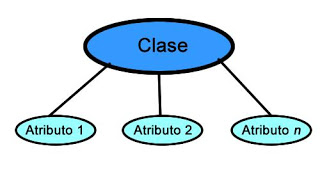
\includegraphics[scale=0.6]{nive}
\par\end{centering}
\caption{Representación gráfica del algoritmo Naive Bayes.}
\end{figure}
Se ejecutó el algoritmo Naive Bayes en Weka para crear los clasificadores de las distintas vistas minables. Los resultados se muestran en la tabla \ref{tab:cuadro36}

\begin{longtable}{|p{3cm}|p{3cm}|p{2cm}|p{2cm}|p{2cm}|p{2cm}|}
%\centering
%\begin{tabular}{|p{3cm}|p{3cm}|p{2cm}|p{2cm}|p{2cm}|p{2cm}|}
\hline
	\rowcolor[gray]{0.5} 
	\multicolumn{2}{|c|}{Vista minable} &
	\multicolumn{4}{|c|}{Porcentaje de éxito de las instancias clasificadas}\\
	\hline
	\rowcolor[gray]{0.9} 
	Nombre & \# de instancias & 100\% & 90\% & 80\% & 70\%\\
	\hline
	\endhead
	\hline
	\multicolumn{6}{r}{\textit{Continua en la siguiente pagina.}} \\
	\endfoot
	\endlastfoot
\multirow{3}[5]{*}{Biologia9} & 1000  & 444   & 479   & 70    & 6 \\
\cline{2-6}      & 10000 & 442   & 480   & 71    & 7 \\
\cline{2-6}      & 100000 & 450   & 478   & 68    & 4 \\
\hline
\multirow{3}[6]{*}{Biologia10} & 1000  & 340   & 475   & 148   & 34 \\
\cline{2-6}      & 10000 & 242   & 423   & 243   & 78 \\
\cline{2-6}      & 100000 & 183   & 325   & 222   & 100 \\
\hline
\multirow{3}[6]{*}{Filosofia7} & 1000  & 374   & 441   & 140   & 38 \\
\cline{2-6}      & 10000 & 287   & 467   & 181   & 47 \\
\cline{2-6}      & 100000 & 226   & 416   & 192   & 92 \\
\hline
\multirow{3}[6]{*}{Fisica11} & 1000  & 348   & 440   & 179   & 28 \\
\cline{2-6}      & 10000 & 259   & 365   & 234   & 108 \\
\cline{2-6}      & 100000 & 185   & 289   & 263   & 193 \\
\hline
\multirow{3}[6]{*}{Fisica112} & 1000  & 340   & 411   & 198   & 46 \\
\cline{2-6}      & 10000 & 229   & 349   & 247   & 131 \\
\cline{2-6}      & 100000 & 192   & 252   & 226   & 214 \\
\hline
\multirow{2}[4]{*}{Ingles11} & 1000  & 441   & 432   & 85    & 17 \\
\cline{2-6}      & 10000 & 452   & 418   & 84    & 14 \\
\hline
\multirow{3}[6]{*}{Lenguaje10} & 1000  & 309   & 454   & 198   & 37 \\
\cline{2-6}      & 10000 & 209   & 347   & 274   & 125 \\
\cline{2-6}      & 100000 & 125   & 224   & 239   & 194 \\
\hline
\multirow{3}[6]{*}{Lenguaje102} & 1000  & 555   & 397   & 46    & 2 \\
\cline{2-6}      & 10000 & 478   & 467   & 52    & 3 \\
\cline{2-6}      & 100000 & 437   & 487   & 68    & 6 \\
\hline
\multirow{3}[6]{*}{Matematica10} & 1000  & 244   & 429   & 187   & 91 \\
\cline{2-6}      & 10000 & 200   & 351   & 205   & 111 \\
\cline{2-6}      & 100000 & 190   & 296   & 197   & 142 \\
\hline
\multirow{3}[6]{*}{Matematica102} & 1000  & 279   & 449   & 197   & 61 \\
\cline{2-6}      & 10000 & 274   & 439   & 217   & 60 \\
\cline{2-6}      & 100000 & 246   & 454   & 214   & 78 \\
\hline
\multirow{3}[6]{*}{MedioAmbiente5} & 1000  & 255   & 582   & 154   & 2 \\
\cline{2-6}      & 10000 & 191   & 540   & 143   & 12 \\
\cline{2-6}      & 100000 & 169   & 486   & 144   & 95 \\
\hline
\multirow{3}[6]{*}{MedioAmbiente7} & 1000  & 205   & 561   & 137   & 13 \\
\cline{2-6}      & 10000 & 123   & 380   & 265   & 122 \\
\cline{2-6}      & 100000 & 78    & 279   & 199   & 219 \\
\hline
\multirow{3}[6]{*}{ProBiologia6} & 1000  & 212   & 398   & 313   & 62 \\
\cline{2-6}      & 10000 & 217   & 398   & 309   & 61 \\
\cline{2-6}      & 50000 & 210   & 401   & 307   & 71 \\
\hline
\multirow{3}[6]{*}{ProBiologia8} & 1000  & 234   & 372   & 299   & 80 \\
\cline{2-6}      & 10000 & 219   & 366   & 286   & 107 \\
\cline{2-6}      & 50000 & 222   & 375   & 279   & 99 \\
\hline
\multirow{3}[6]{*}{ProLenguaje7} & 1000  & 194   & 554   & 227   & 22 \\
\cline{2-6}      & 10000 & 204   & 546   & 235   & 14 \\
\cline{2-6}      & 50000 & 192   & 540   & 246   & 19 \\
\hline
\multirow{3}[6]{*}{ProLenguaje9} & 1000  & 196   & 533   & 242   & 24 \\
\cline{2-6}      & 10000 & 214   & 518   & 244   & 17 \\
\cline{2-6}      & 50000 & 196   & 511   & 251   & 35 \\
\hline
\multirow{3}[6]{*}{ProMatematica7} & 1000  & 262   & 582   & 122   & 25 \\
\cline{2-6}      & 10000 & 290   & 556   & 110   & 32 \\
\cline{2-6}      & 50000 & 339   & 494   & 128   & 30 \\
\hline
\multirow{3}[6]{*}{ProMatematica9} & 1000  & 262   & 536   & 147   & 44 \\
\cline{2-6}      & 10000 & 311   & 501   & 129   & 48 \\
\cline{2-6}      & 50000 & 295   & 504   & 136   & 52 \\
\hline
\multirow{3}[6]{*}{ProSociales7} & 1000  & 166   & 611   & 208   & 12 \\
\cline{2-6}      & 10000 & 214   & 564   & 206   & 14 \\
\cline{2-6}      & 50000 & 210   & 565   & 208   & 13 \\
\hline
\multirow{3}[6]{*}{ProSociales9} & 1000  & 254   & 532   & 192   & 17 \\
\cline{2-6}      & 10000 & 209   & 551   & 224   & 13 \\
\cline{2-6}      & 50000 & 199   & 543   & 227   & 27 \\
\hline
\multirow{3}[6]{*}{Quimica10} & 1000  & 397   & 382   & 187   & 32 \\
\cline{2-6}      & 10000 & 285   & 370   & 238   & 79 \\
\cline{2-6}      & 100000 & 225   & 258   & 232   & 172 \\
\hline
\multirow{3}[6]{*}{Sociales7} & 1000  & 401   & 493   & 94    & 11 \\
\cline{2-6}      & 10000 & 369   & 445   & 150   & 33 \\
\cline{2-6}      & 100000 & 349   & 426   & 162   & 41 \\
\hline
\multirow{3}[6]{*}{Sociales9} & 1000  & 332   & 484   & 146   & 34 \\
\cline{2-6}      & 10000 & 263   & 424   & 254   & 50 \\
\cline{2-6}      & 100000 & 186   & 358   & 245   & 104 \\
\hline
\multirow{3}[6]{*}{Violencia11} & 1000  & 295   & 368   & 179   & 82 \\
\cline{2-6}      & 10000 & 214   & 316   & 187   & 137 \\
\cline{2-6}      & 100000 & 160   & 241   & 163   & 181 \\
\hline
\caption{Resultados de la construcción y evaluación de las vistas minables usando el algoritmo Naive Bayes.}
\label{tab:cuadro36}
\end{longtable}
Este algoritmo a diferencia de los anteriores mostró una menor confianza, por encima del 80\% de precisión estaban, en general, alrededor de 70\% de las instancias evaluadas, pero algunos clasificadores si tuvieron un nivel de confianza mayor.

En general el algoritmo presenta muchas variaciones en sus clasificaciones y por tanto su confianza no es tan acertada como lo fue, por ejemplo, la del algoritmo de los k vecinos más cercanos.
\subsection{Funciones de base radial}
El algoritmo de creación de clasificadores utilizando la red de Funciones de Base Radial o RBF (Radial Basis Function) se encuentra implementado en Weka en la librería RBFNetwork\footnote{\url{ http://weka.sourceforge.net/doc.stable/weka/classifiers/functions/RBFNetwork.html}}.

Las redes neuronales artificiales (RNA) tienen distintas aplicaciones, entre ellas se encuentra la clasificación \cite{key-250}. Su objetivo es tratar de emular la capacidad humana de procesar información.  

Las RNA pueden ser entrenadas usando métodos de aprendizaje supervisado o no supervisado \cite{key-240}. Una de las redes encontradas en el aprendizaje supervisado es la red de Funciones de Base Radial. Las redes RBF constan de 3 capas, en la primera se reciben los atributos de entrada a ser clasificados, en la segunda capa o capa oculta se utiliza una función de calculo para realizar la transformación, no lineal, desde el espacio de la capa de entrada al espacio de la capa intermedia. En la tercera capa se encuentra los valores posibles de la clase a clasificar. 

\begin{figure}[H]
\begin{centering}
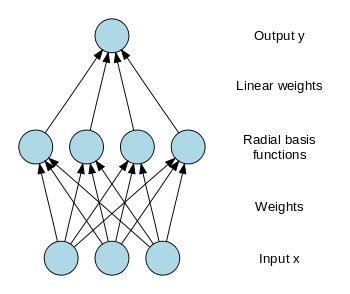
\includegraphics[scale=0.6]{rbf}
\par\end{centering}
\caption{Estructura de las capas de una red neuronal de funciones de base radial.}
\end{figure}
Se realizo la creación de los clasificadores utilizando las vistas minables. Los resultados se muestran en la tabla \ref{tab:cuadro37}

\begin{longtable}{|p{3cm}|p{3cm}|p{2cm}|p{2cm}|p{2cm}|p{2cm}|}
%\centering
%\begin{tabular}{|p{3cm}|p{3cm}|p{2cm}|p{2cm}|p{2cm}|p{2cm}|}
\hline
	\rowcolor[gray]{0.5} 
	\multicolumn{2}{|c|}{Vista minable} &
	\multicolumn{4}{|c|}{Porcentaje de éxito de las instancias clasificadas}\\
	\hline
	\rowcolor[gray]{0.9} 
	Nombre & \# de instancias & 100\% & 90\% & 80\% & 70\%\\
	\hline
	\endhead
	\hline
	\multicolumn{6}{r}{\textit{Continua en la siguiente pagina.}} \\
	\endfoot
	\endlastfoot
\multirow{3}[5]{*}{Biologia9} & 1000  & 434   & 485   & 73    & 7 \\
\cline{2-6}      & 10000 & 456   & 486   & 52    & 5 \\
\cline{2-6}      & 100000 & 466   & 477   & 52    & 2 \\
\hline
\multirow{3}[6]{*}{Biologia10} & 1000  & 347   & 439   & 120   & 63 \\
\cline{2-6}      & 10000 & 362   & 441   & 151   & 29 \\
\cline{2-6}      & 100000 & 422   & 427   & 96    & 14 \\
\hline
\multirow{3}[6]{*}{Filosofia7} & 1000  & 309   & 448   & 192   & 45 \\
\cline{2-6}      & 10000 & 376   & 476   & 97    & 30 \\
\cline{2-6}      & 100000 & 382   & 497   & 98    & 22 \\
\hline
\multirow{3}[6]{*}{Fisica11} & 1000  & 273   & 321   & 92    & 78 \\
\cline{2-6}      & 10000 & 408   & 445   & 110   & 34 \\
\cline{2-6}      & 100000 & 523   & 396   & 68    & 9 \\
\hline
\multirow{3}[6]{*}{Fisica112} & 1000  & 416   & 428   & 132   & 21 \\
\cline{2-6}      & 10000 & 473   & 426   & 82    & 16 \\
\cline{2-6}      & 100000 & 441   & 420   & 97    & 32 \\
\hline
\multirow{2}[4]{*}{Ingles11} & 1000  & 407   & 440   & 90    & 28 \\
\cline{2-6}      & 10000 & 440   & 439   & 68    & 18 \\
\hline
\multirow{3}[6]{*}{Lenguaje10} & 1000  & 258   & 385   & 289   & 60 \\
\cline{2-6}      & 10000 & 443   & 420   & 86    & 35 \\
\cline{2-6}      & 100000 & 459   & 366   & 97    & 58 \\
\hline
\multirow{3}[6]{*}{Lenguaje102} & 1000  & 507   & 409   & 70    & 11 \\
\cline{2-6}      & 10000 & 567   & 389   & 42    & 2 \\
\cline{2-6}      & 100000 & 563   & 408   & 27    & 2 \\
\hline
\multirow{3}[6]{*}{Matematica10} & 1000  & 216   & 380   & 195   & 85 \\
\cline{2-6}      & 10000 & 296   & 504   & 147   & 45 \\
\cline{2-6}      & 100000 & 340   & 520   & 109   & 18 \\
\hline
\multirow{3}[6]{*}{Matematica102} & 1000  & 317   & 449   & 171   & 43 \\
\cline{2-6}      & 10000 & 342   & 480   & 142   & 24 \\
\cline{2-6}      & 100000 & 355   & 494   & 117   & 24 \\
\hline
\multirow{3}[6]{*}{MedioAmbiente5} & 1000  & 183   & 677   & 121   & 0 \\
\cline{2-6}      & 10000 & 196   & 668   & 127   & 0 \\
\cline{2-6}      & 100000 & 166   & 679   & 83    & 32 \\
\hline
\multirow{3}[6]{*}{MedioAmbiente7} & 1000  & 242   & 643   & 81    & 1 \\
\cline{2-6}      & 10000 & 257   & 644   & 86    & 5 \\
\cline{2-6}      & 100000 & 135   & 640   & 137   & 20 \\
\hline
\multirow{3}[6]{*}{ProBiologia6} & 1000  & 200   & 390   & 301   & 94 \\
\cline{2-6}      & 10000 & 242   & 410   & 280   & 55 \\
\cline{2-6}      & 50000 & 262   & 419   & 274   & 36 \\
\hline
\multirow{3}[6]{*}{ProBiologia8} & 1000  & 233   & 366   & 277   & 96 \\
\cline{2-6}      & 10000 & 268   & 396   & 259   & 62 \\
\cline{2-6}      & 50000 & 281   & 397   & 253   & 59 \\
\hline
\multirow{3}[6]{*}{ProLenguaje7} & 1000  & 211   & 546   & 209   & 28 \\
\cline{2-6}      & 10000 & 199   & 559   & 229   & 12 \\
\cline{2-6}      & 50000 & 208   & 560   & 221   & 10 \\
\hline
\multirow{3}[6]{*}{ProLenguaje9} & 1000  & 226   & 531   & 227   & 9 \\
\cline{2-6}      & 10000 & 217   & 548   & 222   & 8 \\
\cline{2-6}      & 50000 & 220   & 543   & 222   & 9 \\
\hline
\multirow{3}[6]{*}{ProMatematica7} & 1000  & 279   & 561   & 111   & 31 \\
\cline{2-6}      & 10000 & 309   & 568   & 90    & 22 \\
\cline{2-6}      & 50000 & 268   & 622   & 78    & 23 \\
\hline
\multirow{3}[6]{*}{ProMatematica9} & 1000  & 315   & 499   & 130   & 36 \\
\cline{2-6}      & 10000 & 248   & 574   & 96    & 38 \\
\cline{2-6}      & 50000 & 251   & 606   & 98    & 35 \\
\hline
\multirow{3}[6]{*}{ProSociales7} & 1000  & 188   & 565   & 211   & 30 \\
\cline{2-6}      & 10000 & 191   & 584   & 208   & 12 \\
\cline{2-6}      & 50000 & 181   & 613   & 192   & 10 \\
\hline
\multirow{3}[6]{*}{ProSociales9} & 1000  & 244   & 524   & 206   & 19 \\
\cline{2-6}      & 10000 & 185   & 599   & 204   & 9 \\
\cline{2-6}      & 50000 & 177   & 608   & 203   & 7 \\
\hline
\multirow{3}[6]{*}{Quimica10} & 1000  & 431   & 411   & 126   & 28 \\
\cline{2-6}      & 10000 & 450   & 394   & 141   & 14 \\
\cline{2-6}      & 100000 & 459   & 424   & 77    & 26 \\
\hline
\multirow{3}[6]{*}{Sociales7} & 1000  & 370   & 486   & 125   & 17 \\
\cline{2-6}      & 10000 & 377   & 419   & 96    & 30 \\
\cline{2-6}      & 100000 & 469   & 434   & 87    & 7 \\
\hline
\multirow{3}[6]{*}{Sociales9} & 1000  & 369   & 505   & 114   & 8 \\
\cline{2-6}      & 10000 & 413   & 462   & 112   & 12 \\
\cline{2-6}      & 100000 & 398   & 480   & 93    & 19 \\
\hline
\multirow{3}[6]{*}{Violencia11} & 1000  & 268   & 380   & 200   & 86 \\
\cline{2-6}      & 10000 & 374   & 423   & 129   & 45 \\
\cline{2-6}      & 100000 & 323   & 380   & 161   & 91 \\
\hline
\caption{Resultados de la construcción y evaluación de las vistas minables usando el algoritmo RBF.}
\label{tab:cuadro37}
\end{longtable}
En los clasificadores construidos con redes RBF se puede notar de nuevo una mejora en la calidad de la predicciones. Al momento de clasificar las instancias de entrenamiento, en todos los clasificadores construidos se logra una predicción del 80\% de precisión en más del 90\% de las instancias de evaluación.

También en este clasificador se observó una tendencia más marcada en algunos clasificadores a mejorar la calidad de sus precisiones a medida que se incrementaba la cantidad de instancias de entrenamientos. 

En conclusión, los clasificadores con este algoritmo, también generaron una buena confianza con la calidad de sus resultados.
\section{Selección de los clasificadores}
Teniendo en cuenta los resultados que obtuvieron cada uno de los clasificadores con cada una de las vistas minables presentadas por las áreas académicas, se eligieron los mejores resultados por cada una.

La elección de los mejores clasificadores se realizó comparando primero cuál de los clasificadores clasificaba más instancias con un 100\% de precisión, si existían 2 o más con la misma cantidad de instancias en este valor, se elegía el que tuviera más instancias clasificadas con un 90\% de precisión y así sucesivamente.

Teniendo en cuenta este criterio y los resultados relacionados en las tablas anteriores, los clasificadores seleccionados se relacionan en la tabla \ref{tab:cuadro38}.

\begin{table}[!Hhtb]
\centering
\begin{tabular}{|p{6.5cm}|p{3cm}|p{3cm}|p{3cm}|}
\hline
	\rowcolor[gray]{0.9} 
	\textbf{Área académica} &
	\textbf{Vista minable} &
	\textbf{Instancias de entrenamiento} &
	\textbf{Algoritmo del clasificador}
	\\
\hline
Biología & Biologia9 & 100.000 & Redes RBF \\
\hline
Ciencias Sociales & Sociales7 & 100.000 & Redes RBF \\
\hline
Filosofia & Filosofia7 & 10.000 & KNN K=2 \\
\hline
Fisica & Fisica11 & 100.000 & Redes RBF \\
\hline
Ingles & Ingles11 & 10.000 & KNN K=2 \\
\hline
Lenguaje & Lenguaje102 & 10.000 & Redes RBF \\
\hline
Matematica & Matematica10 & 10.000 & KNN K=1 \\
\hline
Medio Ambiente & MedioAmbiente5 & 1.000 & Naive Bayes \\
\hline
Profundizacion en Biologia & ProBiologia8 & 100.000 & Redes RBF \\
\hline
Profundizacion en Lenguaje & ProLenguaje9 & 1.000 & KNN K=2 \\
\hline
Profundizacion en Matematica & ProMatematica7 & 1.000 & KNN K=2 \\
\hline
Profundizacion en Ciencias Sociales & ProSociales7 & 1.000 & KNN K=2 \\
\hline
Quimica & Quimica10 & 10.000 & KNN K=1 \\
\hline
Violencia y Sociedad & Violencia11 & 10.000 & Redes RBF \\
\hline
\end{tabular}
\caption{Clasificadores seleccionados para la construcción de la interfaz de consultas.}
\label{tab:cuadro38}
\end{table}